\chapter{Workloads}
\label{sec:workloads}

%%%%%%%%%%%%%%%%%%%%%%%%%%%%%%%%%%%%%%%%%%%%%%%%%%%%%%%%%%%%%%%%%%%%%%%%%%%%%%
%%%%%%%%%%%%%%%%%%%%%%%%%%%%%%%%%%%%%%%%%%%%%%%%%%%%%%%%%%%%%%%%%%%%%%%%%%%%%%
%%%%%%%%%%%%%%%%%%%%%%%%%%%%%%%%%%%%%%%%%%%%%%%%%%%%%%%%%%%%%%%%%%%%%%%%%%%%%%

\section{Query Description Format}
\label{sub:queries_structure}

Queries are described in natural language using a well-defined structure that consists of three sections:
\textit{description}, a concise textual description of the query,
\textit{parameters}, a list of input parameters and their types;
\textit{results}, a list of expected results and their types.
Additionally, queries returning multiple results specify \emph{sorting criteria} and a \emph{limit} (to return top-$k$ results).
For strings, the sorting criteria should be interpreted as a binary comparison of the strings.%
\footnote{\texttt{C} or \texttt{POSIX} collation in PostgreSQL, see \url{https://www.postgresql.org/docs/13/locale.html}}%
\footnote{\texttt{BINARY} collation in DuckDB, see \url{https://duckdb.org/docs/sql/expressions/collations}}

We use the following notation:

\begin{itemize}
	\item \textbf{Node type}: node type in the dataset.
		One word, possibly constructed by appending multiple words together, starting with an uppercase character and following the camel case notation,
        \eg \textsf{TagClass} represents an entity of type ``TagClass''.
    \item \textbf{Edge type}: edge type in the dataset.
        One word, possibly constructed by appending multiple words together, starting with a lowercase character and following the camel case notation
        \eg \mbox{\textsf{workAt}} represents an edge of type ``workAt''.
    \item \textbf{Attribute}: attribute of a node or an edge in the dataset.
        One word, possibly constructed by appending multiple words together, starting with a lowercase character and following the camel case notation,
        and prefixed by a ``.'' to dereference the node/edge,
        \eg \textsf{person.firstName} refers to ``firstName'' attribute on the ``person'' entity,
        and \mbox{\textsf{studyAt.classYear}} refers to ``classYear'' attribute on the ``studyAt'' edge.
    \item \textbf{Unordered Set}: an unordered collection of distinct elements.
        Surrounded by \{ and \} braces, with the element type between them,
        \eg \textsf{\{String\}} refers to a set of strings.
    \item \textbf{Ordered List}: an ordered collection where duplicate elements are allowed.
        Surrounded by [ and ] braces, with the element type between them,
        \eg \textsf{[String]} refers to a list of strings.
    \item \textbf{Ordered Tuple}: a fixed-length, fixed-order list of elements, where elements at each position of the tuple have predefined, possibly different, types.
        Surrounded by < and > braces, with the element types between them in a specific order
        \eg \textsf{<String, Boolean>} refers to a 2-tuple containing a string value in the first element and a boolean value in the second,
        and \textsf{[<String, Boolean>]} is an ordered list of those 2-tuples.
\end{itemize}

\paragraph{Categorization of results.}

Results are categorized according to their source of origin:

\begin{itemize}
	\item \textbf{Raw} (\texttt{R}), if the result attribute is returned with an unmodified value and type.
	\item \textbf{Calculated} (\texttt{C}), if the result is calculated from attributes using arithmetic operators, functions, boolean conditions, etc.
	\item \textbf{Aggregated} (\texttt{A}), if the result is an aggregated value, \eg a count or a sum of another value. If a result is both calculated and aggregated (\eg \lstinline{count(x) + count(y)} or \lstinline{avg(x + y)}), it is considered an aggregated result.
	\item \textbf{Meta} (\texttt{M}), if the result is based on type information, \eg the type of a node.
\end{itemize}


%%%%%%%%%%%%%%%%%%%%%%%%%%%%%%%%%%%%%%%%%%%%%%%%%%%%%%%%%%%%%%%%%%%%%%%%%%%%%%
%%%%%%%%%%%%%%%%%%%%%%%%%%%%%%%%%%%%%%%%%%%%%%%%%%%%%%%%%%%%%%%%%%%%%%%%%%%%%%
%%%%%%%%%%%%%%%%%%%%%%%%%%%%%%%%%%%%%%%%%%%%%%%%%%%%%%%%%%%%%%%%%%%%%%%%%%%%%%

\section{Conventions for Query Definitions}

\paragraph{Interval notations.}

Closed interval boundaries are denoted with 
\texttt{[} 
and \texttt{]}, while open interval boundaries are denoted with \texttt{(} and 
\texttt{)}. For example, \texttt{[0, 1)} denotes an interval between 0 and 1, 
closed on the left and open on the right.

\paragraph{Comparing Date and DateTime values.}

Some query specifications (\eg \queryRefCard{bi-read-01}{BI}{1}) require implementations to compare a
\textsf{DateTime} value with a \textsf{Date} value. In these cases, the 
\textsf{Date} value should be implicitly converted \textsf{DateTime} value 
with a time of 00:00:00.000+00:00 (\ie with the timezone of GMT).

\paragraph{Matching semantics.}

Unless noted otherwise, the specification uses \emph{homomorphic} matching 
semantics~\cite{DBLP:journals/csur/AnglesABHRV17}, \ie both nodes and edges can 
occur multiple times in a match. Note that for variable-length path, duplicate 
edges are not allowed.

\paragraph{Aggregation semantics.}

The \lstinline{count} aggregation always requires the query to determine the number of \emph{distinct} elements (nodes or edges). For example, this can be achieved in the Cypher, SPARQL and SQL query languages with the \lstinline[language=sql]{count(DISTINCT ...)} construct.

\paragraph{Graph patterns.}

To illustrate queries, we use graph patterns such as \autoref{fig:example-graph-pattern} with the following notation:

\begin{figure}[ht]
	\begin{center}
		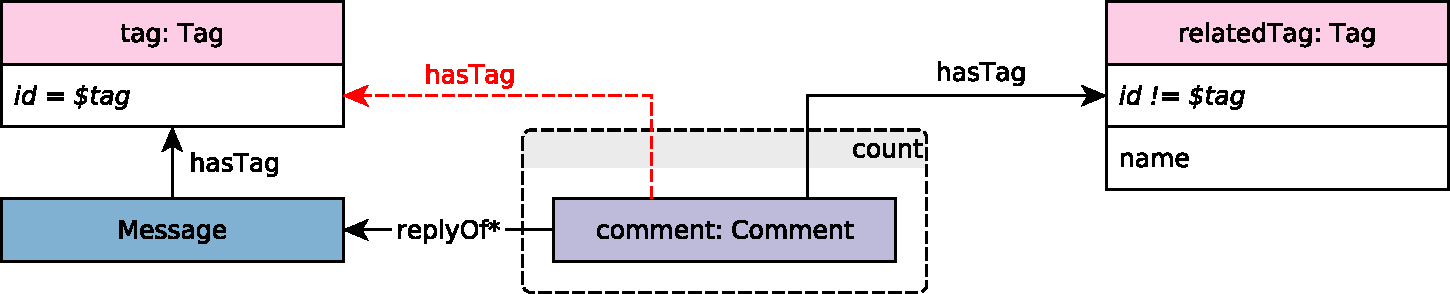
\includegraphics[scale=\yedscale,margin=0cm .2cm]{patterns/bi-read-08}
		\caption{Example graph pattern.}
		\label{fig:example-graph-pattern}
	\end{center}
\end{figure}

\begin{itemize}
	\item Nodes in the pattern are shown with rectangular boxes with their type name stated at the top and emphasized with colour coding.
	\item A black square $\blacksquare$ in the node's top left corner and a \emph{\textbf{bold italic}} condition denote that the node is uniquely specified by the query parameters (\eg by using an identifier or a unique attribute such as \textsf{URL}).
	\item Attributes of nodes and edges can be subject to range constraints (\eg date within a given range, birthday larger than a given date, \etc). These are denoted with the \raisebox{0.3ex}{$\blacktriangledown$} symbol.
	\item Nodes in the pattern are captioned with \textsf{entityName: EntityType} (camel case 
	notation for both, starting with a lowercase character for the first and an 
	uppercase character for the second). If the \textsf{entityName} is neither returned in the query results (in raw, aggregated, or calculated form), nor referenced in the query specification, the \textsf{entityName} can be omitted.
	\item Edges in the graph pattern use the following notation:
	\begin{itemize}
		\item Regular edges, \ie edges that must be present in the subgraph, are denoted with \uline{solid black lines}.
		\item Negative edges, \ie edges that must not be present in the subgraph, are denoted with \textcolor{red}{\dashuline{dashed red lines}} and the \guillemotleft neg\guillemotright\ keyword.
		\item Optional edges, \ie edges that may or may not be in the subgraph, are denoted with \dashuline{dashed black lines}, the \guillemotleft opt\guillemotright\ keyword, and a circle symbol $\circ$ at the optional end of the edge.
		\item Edges without direction have no arrows. Their semantics is that there must be an edge in \emph{the least one of the (incoming, outgoing) directions}.
	\end{itemize}
	\begin{center}
		\tikzstyle{vertex} = [rectangle,minimum height=3mm,minimum width=6mm]
		\begin{tikzpicture}[node distance=15mm]
		\node[draw] (v1) [vertex] {};
		\node[draw] (v2) [vertex,right of=v1] {};
		\draw[solid,->,>=stealth]
		(v1) -- node [midway,above] {} (v2);
		\end{tikzpicture}
		\qquad
		\tikzstyle{vertex} = [rectangle,minimum height=3mm,minimum width=6mm]
		\begin{tikzpicture}[node distance=15mm]
		\node[draw] (v1) [vertex] {};
		\node[draw] (v2) [vertex,right of=v1] {};
		\draw[densely dashed,->,>=stealth,color=red]
		(v1) -- node [midway,above] {\scriptsize{\guillemotleft neg\guillemotright}} (v2);
		\end{tikzpicture}
		\qquad
		\tikzstyle{vertex} = [rectangle,minimum height=3mm,minimum width=6mm]
		\begin{tikzpicture}[node distance=15mm]
		\node[draw] (v1) [vertex] {};
		\node[draw] (v2) [vertex,right of=v1] {};
		\draw[densely dashed,o->,>=stealth]
		(v1) -- node [midway,above] {\scriptsize{\guillemotleft opt\guillemotright}} (v2);
		\end{tikzpicture}
		\qquad
		\tikzstyle{vertex} = [rectangle,minimum height=3mm,minimum width=6mm]
		\begin{tikzpicture}[node distance=15mm]
		\node[draw] (v1) [vertex] {};
		\node[draw] (v2) [vertex,right of=v1] {};
		\draw[-]
		(v1) -- node [midway,above] {} (v2);
		\end{tikzpicture}
	\end{center}
	\item Edges with many-to-many cardinalities are denoted with thicker lines, emphasizing that they may contribute more results in the result set.
	\item Filtering conditions are typeset in \textit{italic}, \eg $\textit{id = 
	\textdollar tag}$.
	\item Attributes that should be returned are denoted in sans-serif font, \eg \textsf{name}.
	\item Variable length paths, \ie edges that can be traversed multiple times 
	are denoted with \textsf{*min\ldots{}max}, \eg \textsf{replyOf*} or 
	\textsf{knows*1\ldots{}2}. By default, the value of \textsf{min} is 1, 
	and the value of \textsf{max} is unlimited.
	\item Aggregations are shown in boxes with a grey strip on their top describing the type of aggregation (\lstinline{count}, \lstinline{sum}, \lstinline{average}, etc.).
\end{itemize}

\newcommand{\tuple}[1]{\langle #1 \rangle}

\paragraph{Keywords.} The pattern notation uses a small set of keywords:

\begin{itemize}
	\item Aggregation operations:
	\lstinline{avg},
	\lstinline{count}, 
	\lstinline{sum}.
	\item Functions:
	\begin{itemize}
		\item \lstinline{floor(x)}: returns $\lfloor x \rfloor$,
		\item \lstinline{year(date)}: extracts the year from a given date,
		\item \lstinline{month(date)}: extracts the month from a given date.
		\item \lstinline{day(date)}: extracts the day (of the month) from a given date.
	\end{itemize}
\end{itemize}

\paragraph{Deletions.}
Deletions of a single element are denoted with a red cross~
\includegraphics[scale=0.25]{patterns/delete-single},
while recursive deletions are denoted with a purple cross~
\includegraphics[scale=0.25]{patterns/delete-recursively}.

\paragraph{Resolving ambiguity.}

Note that if the textual description and the graph pattern are different for a particular query (either due to an error or the lack of sophistication in the graphical syntax), \emph{the textual description takes precedence}.

%%%%%%%%%%%%%%%%%%%%%%%%%%%%%%%%%%%%%%%%%%%%%%%%%%%%%%%%%%%%%%%%%%%%%%%%%%%%%%
%%%%%%%%%%%%%%%%%%%%%%%%%%%%%%%%%%%%%%%%%%%%%%%%%%%%%%%%%%%%%%%%%%%%%%%%%%%%%%
%%%%%%%%%%%%%%%%%%%%%%%%%%%%%%%%%%%%%%%%%%%%%%%%%%%%%%%%%%%%%%%%%%%%%%%%%%%%%%

\section{Substitution Parameters}
\label{sec:substitution-parameters}

\input{substitution-parameters}

%%%%%%%%%%%%%%%%%%%%%%%%%%%%%%%%%%%%%%%%%%%%%%%%%%%%%%%%%%%%%%%%%%%%%%%%%%%%%%
%%%%%%%%%%%%%%%%%%%%%%%%%%%%%%%%%%%%%%%%%%%%%%%%%%%%%%%%%%%%%%%%%%%%%%%%%%%%%%
%%%%%%%%%%%%%%%%%%%%%%%%%%%%%%%%%%%%%%%%%%%%%%%%%%%%%%%%%%%%%%%%%%%%%%%%%%%%%%
